% SPDX-License-Identifier: CC-BY-4.0
%
% Copyright (c) 2023 Nelson Vieira
%
% @author Nelson Vieira <2080511@student.uma.pt>
% @contributor Mary Barreto <mary.barreto@staff.uma.pt>
% @license CC-BY-4.0 <https://creativecommons.org/licenses/by/4.0/legalcode.txt>
\section{Results}\label{section:results}

\par
This chapter presents the results of the questionnaire about participants'
perceptions of privacy, \DTLassign{acronyms}{14}{\acronym=Acronym}\hyperlink{\acronym}{\acronym} and theirs online behaviors, as well as the usability
tests that were conducted for the mobile application.

\subsection{Stage 1: Survey}

As would be expected, the majority of participants agreed that data privacy
is important to them and as such should be protected, as can be inferred
in Figure \ref{fig:privacy_is_important_to_me}. Most participants
also have some knowledge of behaviours or techniques to do
in an online environment, as shown in Figure \ref{fig:techniques_to_guarantee_privacy}, be it connected to the internet or on some
local network, like not sharing too much private information
(or none at all) with strangers, revealing only the bare minimum necessary
information to use a particular system, use of \DTLassign{acronyms}{33}{\acronym=Acronym}\hyperlink{\acronym}{\acronym}s (Virtual Private Networks), different and strong
passwords, 2 step authentication methods between others. Because a good
portion of participants are from engineering areas this question might be
skewed.

\begin{figure}[H]
    \begin{center}
        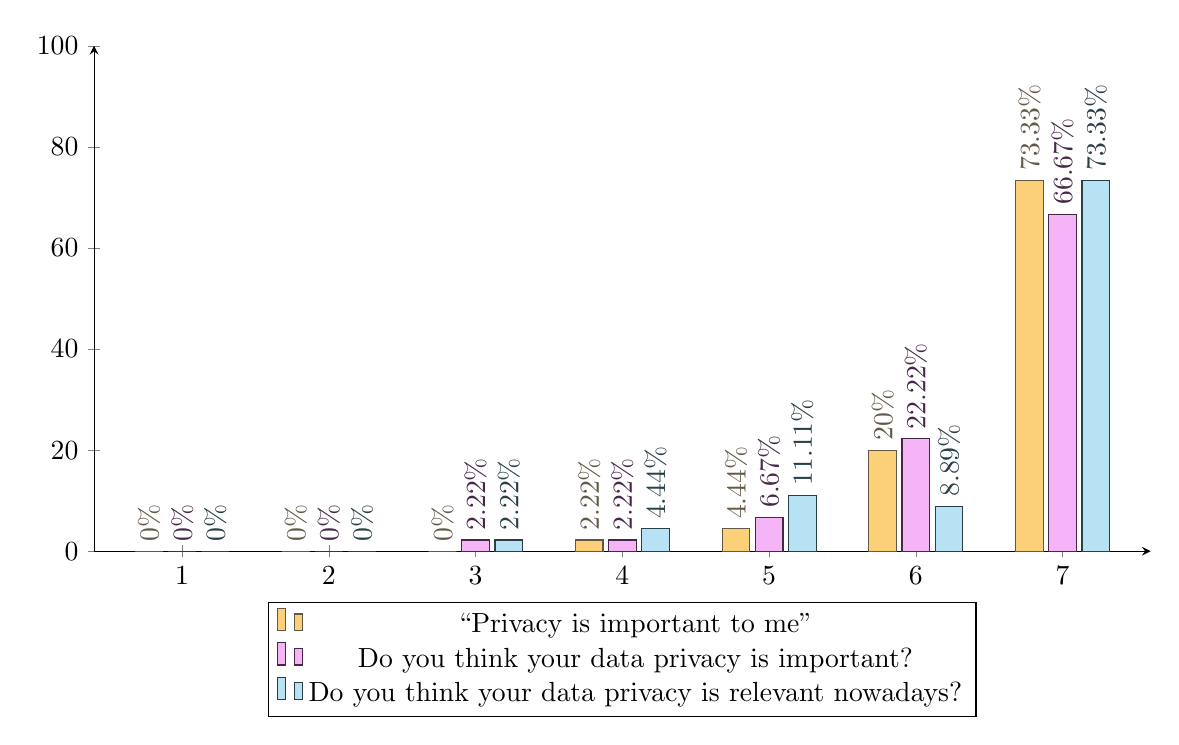
\begin{tikzpicture}
            \begin{axis}[
                height=8cm,
                width=15cm,
                ybar,
                bar width=10pt,
                ymin=0,
                ymax=100,
                xtick=data,
                axis x line=bottom,
                axis y line=left,
                enlarge x limits=0.1,
                nodes near coords={\pgfmathprintnumber\pgfplotspointmeta\%},
                every node near coord/.append style={rotate=90, anchor=west},
                legend style={at={(0.5,-0.1)},anchor=north}
            ]
                \addplot[Dandelion!30!black,fill=Dandelion!60!white] coordinates {(1,0) (2,0) (3,0) (4,2.22) (5,4.44) (6,20) (7,73.33)};
                \addlegendentry{``Privacy is important to me''}
                \addplot[Violet!30!black,fill=Violet!60!white] coordinates {(1,0) (2,0) (3,2.22) (4,2.22) (5,6.67) (6,22.22) (7,66.67)};
                \addlegendentry{Do you think your data privacy is important?}
                \addplot[SkyBlue!30!black,fill=SkyBlue!60!white] coordinates {(1,0) (2,0) (3,2.22) (4,4.44) (5,11.11) (6,8.89) (7,73.33)};
                \addlegendentry{Do you think your data privacy is relevant nowadays?}
            \end{axis}
        \end{tikzpicture}
        \caption{Perspectives of participants on the importance of personal data privacy.}
        \label{fig:privacy_is_important_to_me}
    \end{center}
\end{figure}

\begin{figure}[H]
    \begin{center}
        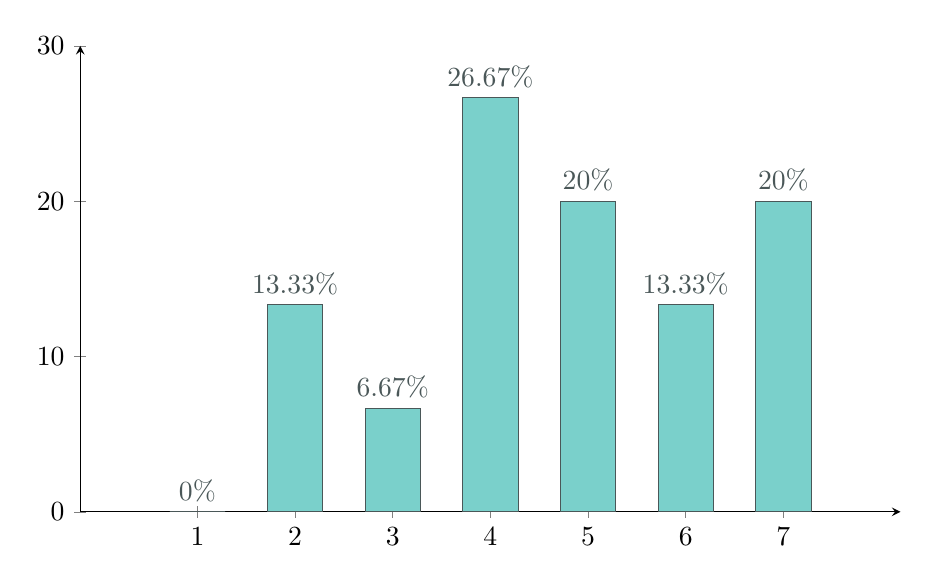
\begin{tikzpicture}
            \begin{axis}[
                height=7.5cm,
                width=12cm,
                ybar,
                bar width=20pt,
                ymin=0,
                ymax=30,
                xtick=data,
                axis x line=bottom,
                axis y line=left,
                enlarge x limits=0.2,
                nodes near coords={\pgfmathprintnumber\pgfplotspointmeta\%}
            ]
                \addplot[TealBlue!30!black,fill=TealBlue!60!white] coordinates {(1,0) (2,13.33) (3,6.67) (4,26.67) (5,20) (6,13.33) (7,20)};
            \end{axis}
        \end{tikzpicture}
        \caption{Participant responses indicating whether they know techniques to guarantee privacy and the protection of their data when using the internet.}
        \label{fig:techniques_to_guarantee_privacy}
    \end{center}
\end{figure}

Most participants consider data privacy as a human and consumer right,
as shown in Figure \ref{fig:privacy_human_right_histogram}, even if they have
no knowledge of article 12 of the Universal Declaration of Human Rights.

\begin{figure}[H]
    \begin{center}
        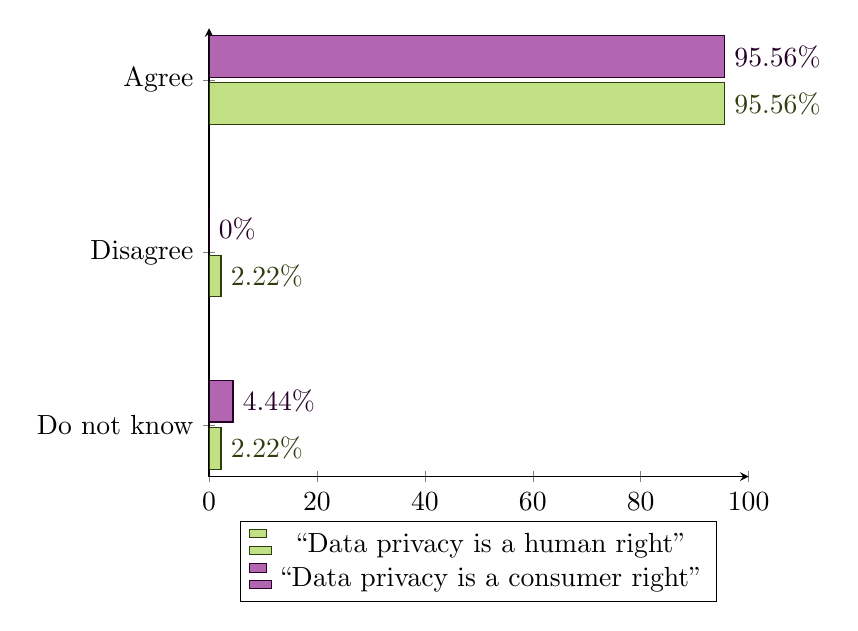
\begin{tikzpicture}
            \begin{axis}[
                xbar,
                symbolic y coords={Do not know,Disagree,Agree},
                bar width=15pt,
                ytick=data,
                axis x line=bottom,
                axis y line=left,
                xmin=0,
                xmax=100,
                enlarge y limits=0.15,
                nodes near coords={\pgfmathprintnumber\pgfplotspointmeta\%},
                legend style={at={(0.5,-0.1)},anchor=north}
            ]
                \addplot[YellowGreen!30!black,fill=YellowGreen!60!white] coordinates {(2.22,Do not know) (2.22,Disagree) (95.56,Agree)};
                \addlegendentry{``Data privacy is a human right''}
                \addplot[Purple!30!black,fill=Purple!60!white] coordinates {(4.44,Do not know) (0,Disagree) (95.56,Agree)};
                \addlegendentry{``Data privacy is a consumer right''}
            \end{axis}
        \end{tikzpicture}
        \caption{Participant responses regarding privacy rights.}
        \label{fig:privacy_human_right_histogram}
    \end{center}
\end{figure}

When asked to define digital privacy, most participants did not know
how to properly define it, giving generic answers while some even gave a one word answer,
some participants gave incomplete or adjacent related answers. Only approximately
16\% of participants supplied a concrete answer that was close to the definition
presented in Chapter \ref{introduction}. Curiously, no one mentioned security,
which contradicts with the responses represented in Figure \ref{fig:security_equals_privacy},
where 53.33\% of participants believe that privacy and security are synonymous.

\begin{figure}[H]
    \centering
    \begin{tikzpicture}
        \pie[explode = 0.1,
            color={OrangeRed!70,YellowGreen!70}
            ]{46.67/No,
            53.33/Yes}
    \end{tikzpicture}
    \caption{Responses to security and privacy being synonymous.}
    \label{fig:security_equals_privacy}
\end{figure}

Participants have some digital literacy of Information Technology \DTLassign{acronyms}{13}{\acronym=Acronym}(\hyperlink{\acronym}{\acronym}) terms, as shown on
Figure \ref{fig:familiar_terms}, most know the more popular
terms like \textit{wi-fi}, \textit{cookie} and \textit{data protection},
but as the terms become more esoteric the general knowledge starts
to drop. Some terms, even after getting some popularity,
are still mostly unknown to the majority of people like \textit{blockchain} or \textit{Internet of Things}.

\begin{figure}[H]
    \begin{center}
        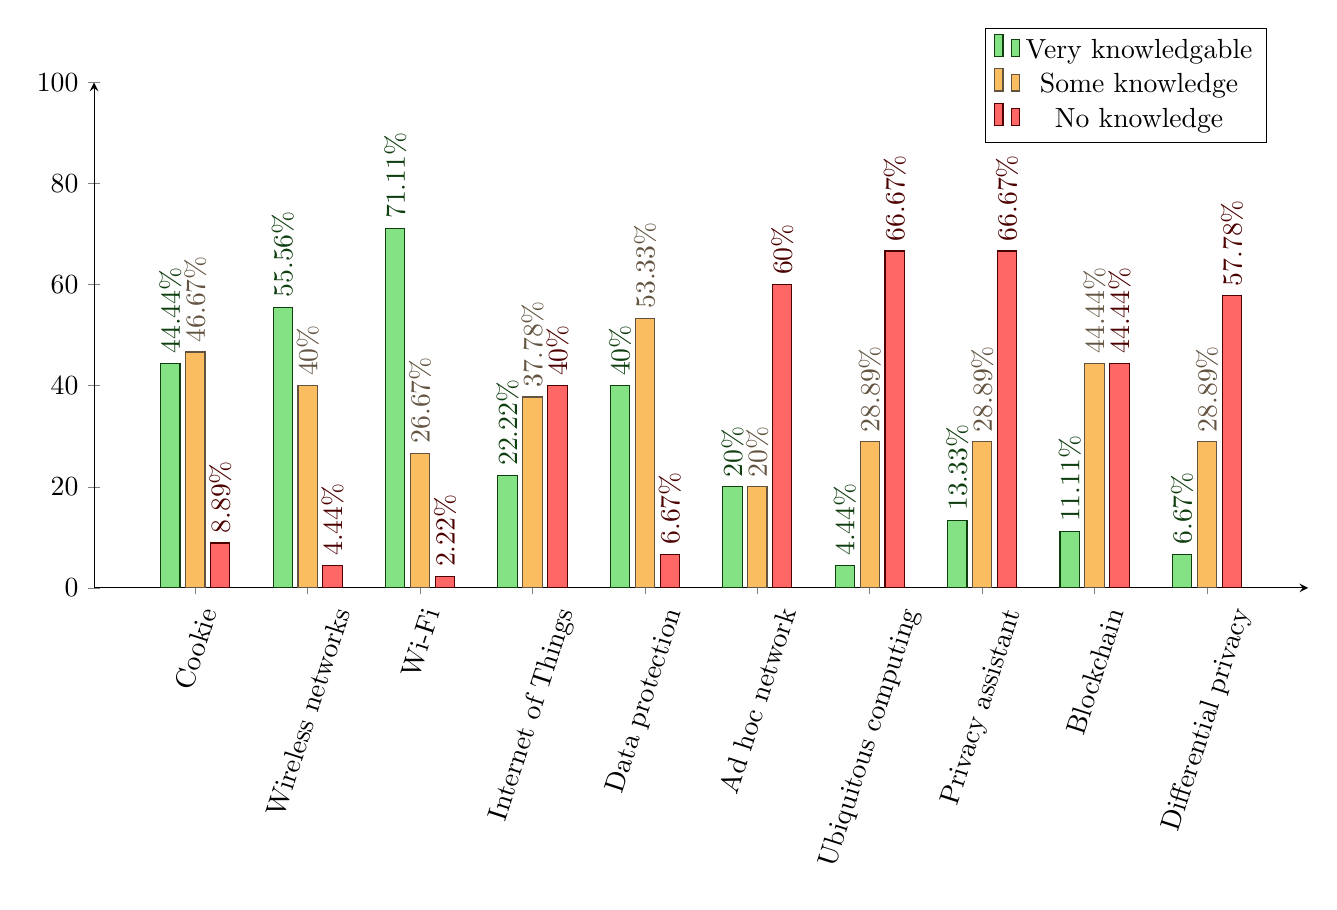
\begin{tikzpicture}
            \begin{axis}[
                height=8cm,
                width=17cm,
                symbolic x coords={Cookie, Wireless networks,Wi-Fi,Internet of Things,Data protection,Ad hoc network,Ubiquitous computing,Privacy assistant,Blockchain,Differential privacy},
                ybar,
                bar width=7pt,
                ymin=0,
                ymax=100,
                xticklabel style={rotate=72},
                axis x line=bottom,
                axis y line=left,
                enlarge x limits=0.1,
                nodes near coords={\pgfmathprintnumber\pgfplotspointmeta\%},
                every node near coord/.append style={rotate=90, anchor=west},
                legend style={at={(0.85,0.88)},anchor=south}
            ]
                \addplot[LimeGreen!30!black,fill=LimeGreen!60!white] coordinates {(Cookie,44.44) (Wireless networks,55.56) (Wi-Fi,71.11) (Internet of Things,22.22) (Data protection,40) (Ad hoc network,20) (Ubiquitous computing,4.44) (Privacy assistant,13.33) (Blockchain,11.11) (Differential privacy,6.67)};
                \addlegendentry{Very knowledgable}
                \addplot[YellowOrange!30!black,fill=YellowOrange!60!white] coordinates {(Cookie,46.67) (Wireless networks,40) (Wi-Fi,26.67) (Internet of Things,37.78) (Data protection,53.33) (Ad hoc network,20) (Ubiquitous computing,28.89) (Privacy assistant,28.89) (Blockchain,44.44) (Differential privacy,28.89)};
                \addlegendentry{Some knowledge}
                \addplot[Red!30!black,fill=Red!60!white] coordinates {(Cookie,8.89) (Wireless networks,4.44) (Wi-Fi,2.22) (Internet of Things,40) (Data protection,6.67) (Ad hoc network,60) (Ubiquitous computing,66.67) (Privacy assistant,66.67) (Blockchain,44.44) (Differential privacy,57.78)};
                \addlegendentry{No knowledge}
            \end{axis}
        \end{tikzpicture}
        \caption{Familiarity with general IT terms.}
        \label{fig:familiar_terms}
    \end{center}
\end{figure}

Regarding users' online habits, all participants have, or have access to, a smartphone
and they use it in their daily lives, most participants concede that they spend a lot
of their daily time using it, like shown in Figure \ref{fig:phone_access}, and are
somewhat worried but do not actively try to protect their data privacy, which
goes against their earlier responses regarding their worry of personal data privacy.
When asked if they accept
cookies, respondents occasionally do but are unsure what they do or their
importance on the user experience.

\begin{figure}[H]
    \begin{center}
        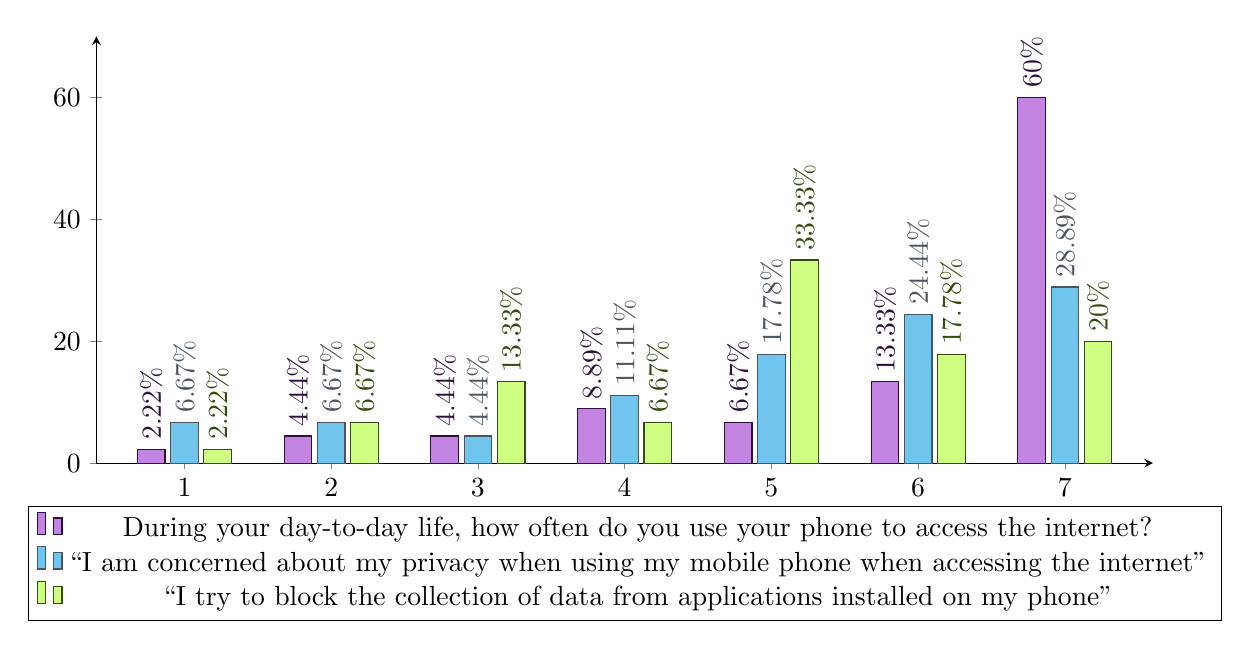
\begin{tikzpicture}
            \begin{axis}[
                height=7cm,
                width=15cm,
                ybar,
                bar width=10pt,
                ymin=0,
                ymax=70,
                % ytick=data,
                xtick=data,
                axis x line=bottom,
                axis y line=left,
                enlarge x limits=0.1,
                nodes near coords={\pgfmathprintnumber\pgfplotspointmeta\%},
                every node near coord/.append style={rotate=90, anchor=west},
                legend style={at={(0.5,-0.1)},anchor=north}
            ]
                \addplot[DarkOrchid!30!black,fill=DarkOrchid!60!white] coordinates {(1,2.22) (2,4.44) (3,4.44) (4,8.89) (5,6.67) (6,13.33) (7,60)};
                \addlegendentry{During your day-to-day life, how often do you use your phone to access the internet?}
                \addplot[Cerulean!30!black,fill=Cerulean!60!white] coordinates {(1,6.67) (2,6.67) (3,4.44) (4,11.11) (5,17.78) (6,24.44) (7,28.89)};
                \addlegendentry{``I am concerned about my privacy when using my mobile phone when accessing the internet''}
                \addplot[GreenYellow!30!black,fill=GreenYellow!60!white] coordinates {(1,2.22) (2,6.67) (3,13.33) (4,6.67) (5,33.33) (6,17.78) (7,20)};
                \addlegendentry{``I try to block the collection of data from applications installed on my phone''}
            \end{axis}
        \end{tikzpicture}
        \caption{Responses related to phone usage.}
        \label{fig:phone_access}
    \end{center}
\end{figure}

% \begin{figure}
%     \begin{center}
%         \begin{tikzpicture}
%             \begin{axis}[
%                 ybar,
%                 xlabel={Agreement level},
%                 ylabel={Responses},
%                 ytick=\empty,
%                 xtick=data,
%                 axis x line=bottom,
%                 axis y line=left,
%                 enlarge x limits=0.2,
%                 bar width=20pt,
%                 nodes near coords={\pgfmathprintnumber\pgfplotspointmeta\%}
%             ]
%                 \addplot coordinates {(1,6.67) (2,2.22) (3,13.33) (4,20) (5,24.44) (6,11.11) (7,22.22)};
%             \end{axis}
%         \end{tikzpicture}
%         \caption{Responses to the question: How often do you allow the use of cookies?}
%         \label{fig:allow_cookies}
%     \end{center}
% \end{figure}

When asked about the concept of profiling, only half of the participants
are aware of the term, but more than half consider that their online
activity contributes to its development, see Figure \ref{fig:activity_contributes_profiling}.

\begin{figure}[H]
    \begin{center}
        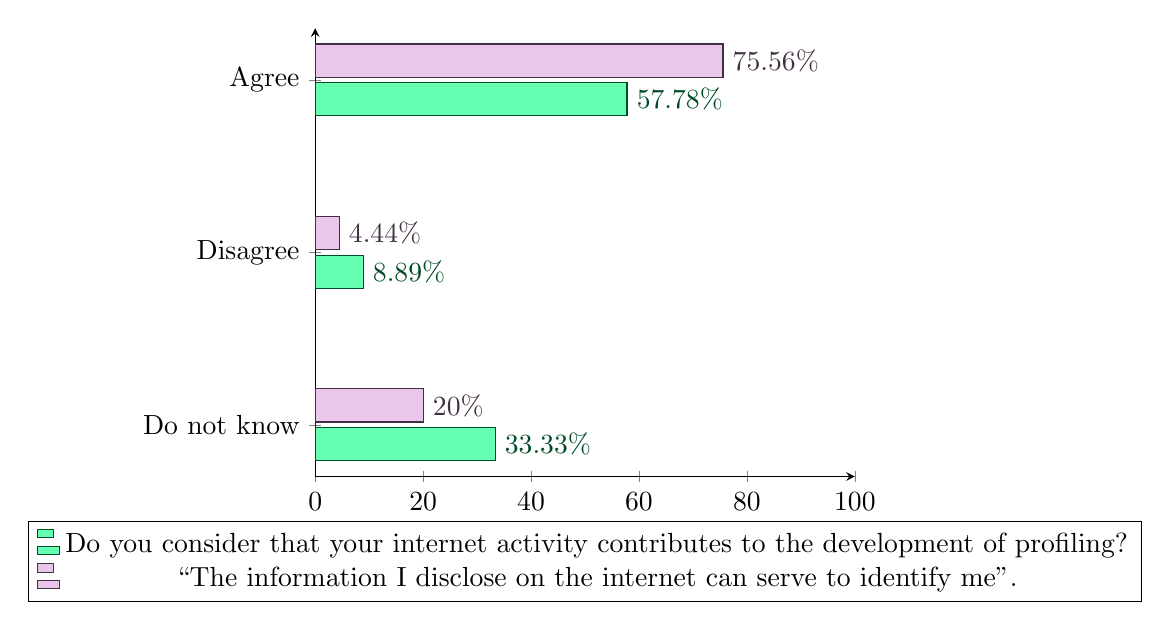
\begin{tikzpicture}
            \begin{axis}[
                xbar,
                symbolic y coords={Do not know,Disagree,Agree},
                bar width=12pt,
                ytick=data,
                axis x line=bottom,
                axis y line=left,
                xmin=0,
                xmax=100,
                enlarge y limits=0.15,
                nodes near coords={\pgfmathprintnumber\pgfplotspointmeta\%},
                legend style={at={(0.5,-0.1)},anchor=north}
            ]
                \addplot[SpringGreen!30!black,fill=SpringGreen!60!white] coordinates {(33.33,Do not know) (8.89,Disagree) (57.78,Agree)};
                \addlegendentry{Do you consider that your internet activity contributes to the development of profiling?}
                \addplot[Plum!30!black,fill=Plum!60!white] coordinates {(20,Do not know) (4.44,Disagree) (75.56,Agree)};
                \addlegendentry{``The information I disclose on the internet can serve to identify me''.}
            \end{axis}
        \end{tikzpicture}
        \caption{Responses from participants with regard to profiling.}
        \label{fig:activity_contributes_profiling}
    \end{center}
\end{figure}

% \begin{figure}
%     \centering
%     \begin{tikzpicture}
%         \pie[explode = 0.1]{33.33/I do not know,
%             8.89/No,
%             57.78/Yes}
%     \end{tikzpicture}
%     \caption{Responses to the question: Do you consider that your internet activity contributes to the development of profiling?}
%     \label{fig:activity_contributes_to_profiling}
% \end{figure}

% \begin{figure}
%     \centering
%     \begin{tikzpicture}
%         \pie[explode = 0.1]{20/I do not know,
%             4.44/No,
%             75.56/Yes}
%     \end{tikzpicture}
%     \caption{Responses to the question: ``The information I disclose on the internet can serve to identify me''. Do you agree with this statement?}
%     \label{fig:information_disclose_internet_identify_me}
% \end{figure}

Regarding participants relation with regulations, most participants are
aware of regulations related to digital privacy, like \DTLassign{acronyms}{9}{\acronym=Acronym}\hyperlink{\acronym}{\acronym} or \DTLassign{acronyms}{3}{\acronym=Acronym}\hyperlink{\acronym}{\acronym}, but
it is not absolutely clear to them what they represent, and they do not
show a clear interest in knowing more about these regulations, as shown in Figure \ref{fig:privacy_regulations}. It is not
clear why there is a certain disinterest by most participants in regulations,
it might be that most find it frustrating to read, or there is some
faith that they work and as such there is no need to know more about them.
Notably 0,47\% of the participants responded correctly to the question
about \DTLassign{acronyms}{9}{\acronym=Acronym}\hyperlink{\acronym}{\acronym}'s definition of personal data.

\begin{figure}[H]
    \begin{center}
        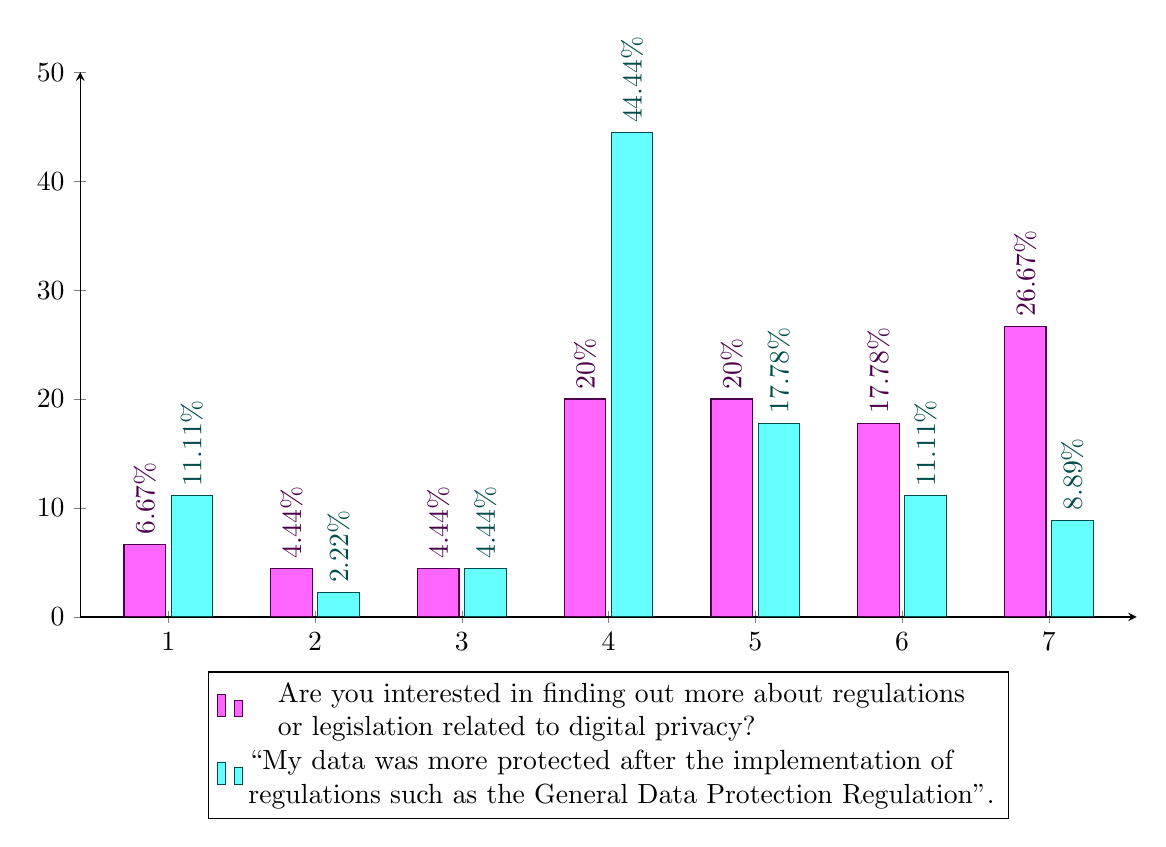
\begin{tikzpicture}
            \begin{axis}[
                height=8.5cm,
                width=15cm,
                ybar,
                bar width=15pt,
                ymin=0,
                ymax=50,
                % ytick=\empty,
                xtick=data,
                % ylabel={Responses \%},
                % xlabel={Agreement level},
                axis x line=bottom,
                axis y line=left,
                enlarge x limits=0.1,
                nodes near coords={\pgfmathprintnumber\pgfplotspointmeta\%},
                every node near coord/.append style={rotate=90, anchor=west},
                legend style={at={(0.5,-0.1)},anchor=north,cells={align=left}}
            ]
                \addplot[Fuchsia!30!black,fill=Fuchsia!60!white] coordinates {(1,6.67) (2,4.44) (3,4.44) (4,20) (5,20) (6,17.78) (7,26.67)};
                \addlegendentry{Are you interested in finding out more about regulations\\or legislation related to digital privacy?}
                \addplot[Cyan!30!black,fill=Cyan!60!white] coordinates {(1,11.11) (2,2.22) (3,4.44) (4,44.44) (5,17.78) (6,11.11) (7,8.89)};
                \addlegendentry{``My data was more protected after the implementation of\\regulations such as the General Data Protection Regulation''.}
            \end{axis}
        \end{tikzpicture}
        \caption{Responses related to privacy regulations.}
        \label{fig:privacy_regulations}
    \end{center}
\end{figure}

% \begin{figure}
%     \begin{center}
%         \begin{tikzpicture}
%             \begin{axis}[
%                 ybar,
%                 xlabel={Agreement level},
%                 ylabel={Responses},
%                 ytick=\empty,
%                 xtick=data,
%                 axis x line=bottom,
%                 axis y line=left,
%                 enlarge x limits=0.2,
%                 bar width=20pt,
%                 nodes near coords={\pgfmathprintnumber\pgfplotspointmeta\%}
%             ]
%                 \addplot coordinates {(1,6.67) (2,4.44) (3,4.44) (4,20) (5,20) (6,17.78) (7,26.67)};
%             \end{axis}
%         \end{tikzpicture}
%         \caption{Responses to the question: Are you interested in finding out more about regulations or legislation related to digital privacy?}
%         \label{fig:finding_out_more_about_regulations}
%     \end{center}
% \end{figure}

% \begin{figure}
%     \begin{center}
%         \begin{tikzpicture}
%             \begin{axis}[
%                 ybar,
%                 ytick=data,
%                 xtick=data,
%                 axis x line=bottom,
%                 axis y line=left,
%                 enlarge x limits=0.2,
%                 bar width=20pt
%             ]
%                 \addplot coordinates {(1,11.11) (2,2.22) (3,4.44) (4,44.44) (5,17.78) (6,11.11) (7,8.89)};
%             \end{axis}
%         \end{tikzpicture}
%         \caption{Responses to the question: ``My data was more protected after the implementation of regulations such as the General Data Protection Regulation''. Do you agree with this statement?}
%         \label{fig:more_protected_after_regulations}
%     \end{center}
% \end{figure}

% \begin{figure}
%     \centering
%     \begin{tikzpicture}
%         \pie[explode = 0.1]{11.11/I disagree,
%             48.89/Maybe if asked first,
%             35.56/I agree}
%     \end{tikzpicture}
%     \caption{Responses to the question: Do you agree to share health data that can identify you with health professionals?}
%     \label{fig:share_health_data_can_identify}
% \end{figure}

% \begin{figure}
%     \centering
%     \begin{tikzpicture}
%         \pie[explode = 0.1]{20/I disagree,
%             35.56/Maybe if asked first,
%             37.78/I agree}
%     \end{tikzpicture}
%     \caption{Responses to the question: Do you agree to share health data that cannot identify you with health professionals?}
%     \label{fig:share_health_data_cannot_identify}
% \end{figure}

Most participants, 73.33\%, do not know what a data protection officer is
or what are their duties, as can be seen in Figure \ref{fig:aware_dpo}.
An internal role known as a data protection officer acts as an independent
spokesman for a company's policies regarding the processing and
application of customer data. The \DTLassign{acronyms}{9}{\acronym=Acronym}\hyperlink{\acronym}{\acronym}, which requires the appointment
of a data protection officer by all businesses that offer goods or
services to consumers in the European Union and collect data as a
result, led to the creation of this job. The data protection officer
keeps up with data protection regulations and policies, conducts
internal privacy audits, and ensures that all other compliance-related
data-related concerns are current.

\begin{figure}[H]
    \centering
    \begin{tikzpicture}
        \pie[explode = 0.1,
            color={RubineRed!70,GreenYellow!70}
            ]{73.33/No,
            26.67/Yes}
    \end{tikzpicture}
    \caption{Awareness of the duties of a data protection officer.}
    \label{fig:aware_dpo}
\end{figure}

As expressed before, participants consider the protection of private data important
and as such 82.22\% are interested in knowing where and how their data is used by
organizations, as shown in Figure \ref{fig:interested_where_how_information_used}.

\begin{figure}
    \centering
    \begin{tikzpicture}
        \pie[explode = 0.1,
            color={Red!60!white,CadetBlue!60!white,LimeGreen!60!white}
            ]{2.22/I disagree,
            15.56/I do not agree nor disagree,
            82.22/I agree}
    \end{tikzpicture}
    \caption{Interest in knowing where and how personal information is used by organizations.}
    \label{fig:interested_where_how_information_used}
\end{figure}

Questions related to privacy notices are displayed in Figure \ref{fig:privacy_notices}.
Participants are interested in knowing how their data is used by organizations,
and privacy notices are one way to convey such information, but not all privacy
notices are created equal, specially in the \DTLassign{acronyms}{14}{\acronym=Acronym}\hyperlink{\acronym}{\acronym}, yet 53.33\% are not familiar with
the reason data is collected but are still curious. Most participants agree that
lengthy texts and font size, 86.67\% and 77.78\% respectively, affect their
willingness to read them, 71.11\% confess to agreeing to the notices just to use
the service due to a fear of missing out. In regard to brand trust, participants
are divided with 33.33\% agreeing to not reading the privacy notice if they trust
the organization and 33.33\% disagreeing.

\begin{figure}[H]
    \begin{center}
        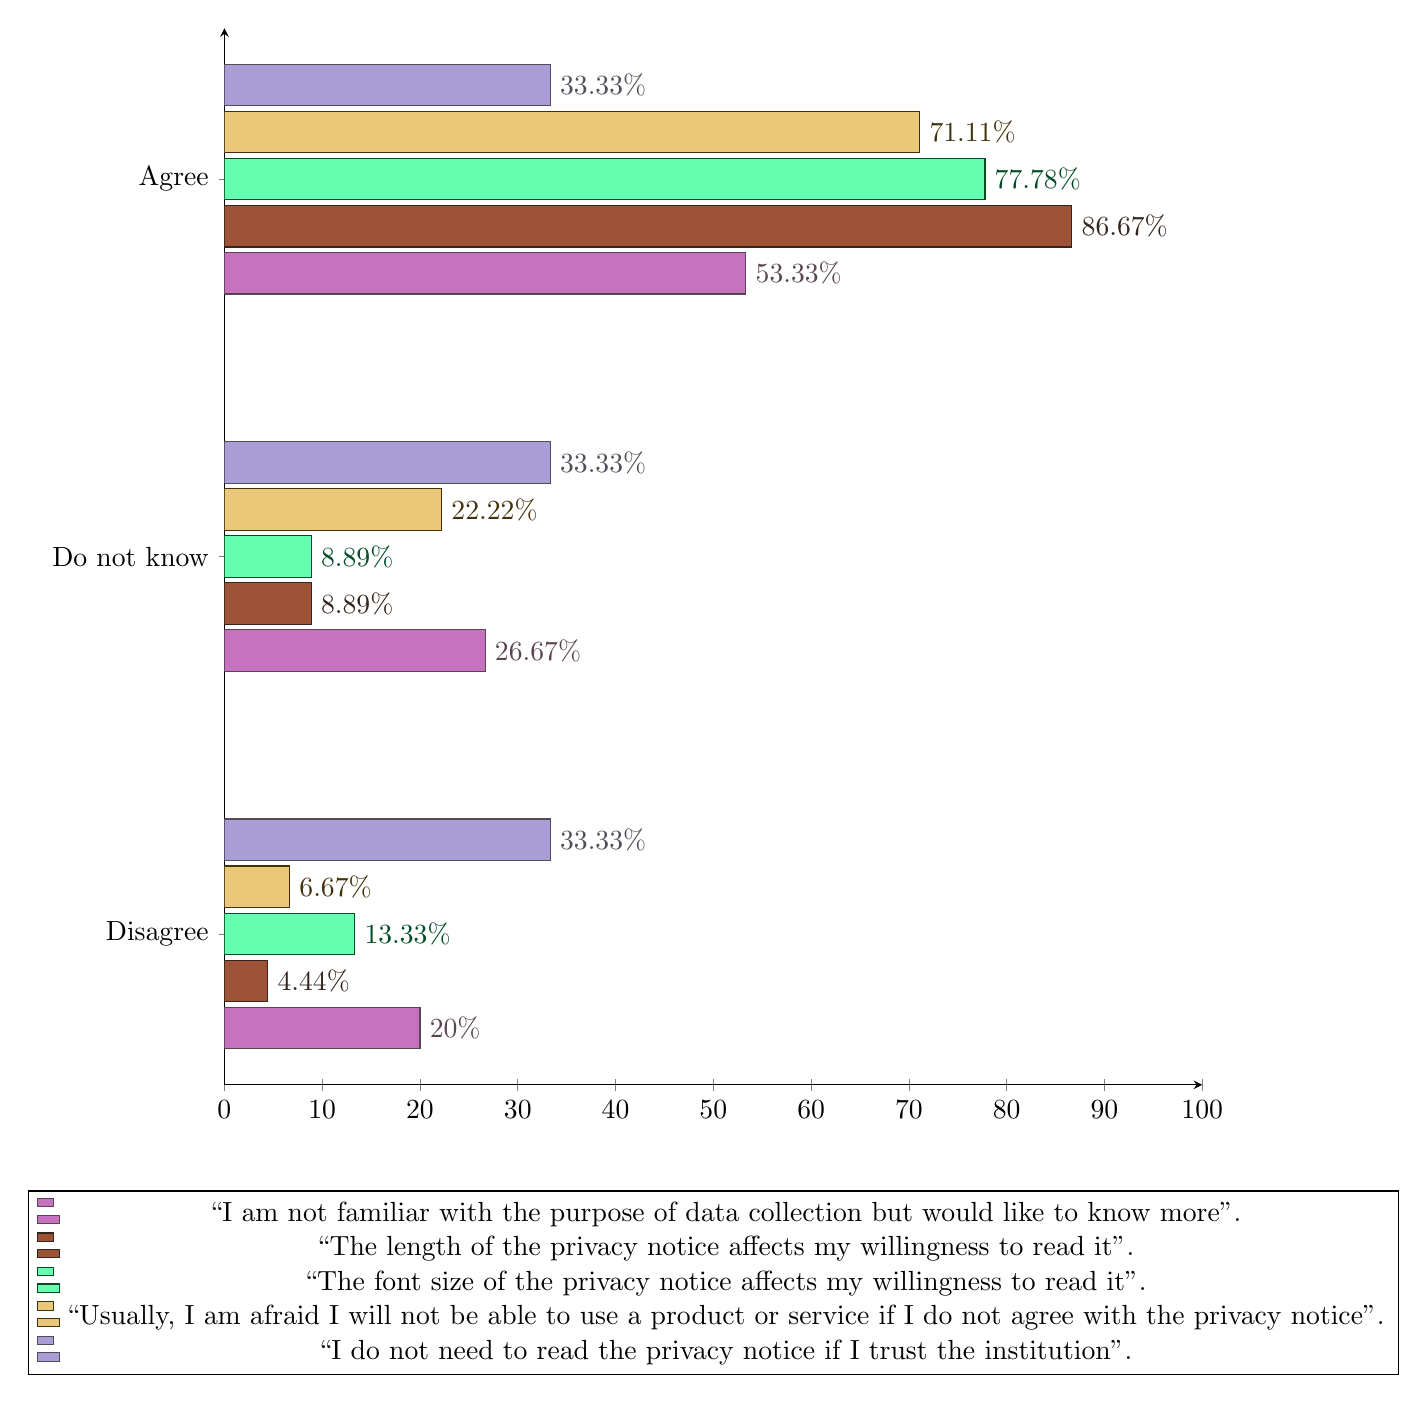
\begin{tikzpicture}
            \begin{axis}[
                height=15cm,
                width=14cm,
                xbar,
                symbolic y coords={Disagree,Do not know,Agree},
                bar width=15pt,
                ytick=data,
                axis x line=bottom,
                axis y line=left,
                xmin=0,
                xmax=100,
                enlarge y limits=0.2,
                nodes near coords={\pgfmathprintnumber\pgfplotspointmeta\%},
                legend style={at={(0.5,-0.1)},anchor=north}
            ]
                \addplot[Mulberry!30!black,fill=Mulberry!60!white] coordinates {(20,Disagree) (26.67,Do not know) (53.33,Agree)};
                \addlegendentry{``I am not familiar with the purpose of data collection but would like to know more''.}
                \addplot[Sepia!30!black,fill=Sepia!60!white] coordinates {(4.44,Disagree) (8.89,Do not know) (86.67,Agree)};
                \addlegendentry{``The length of the privacy notice affects my willingness to read it''.}
                \addplot[SpringGreen!30!black,fill=SpringGreen!60!white] coordinates {(13.33,Disagree) (8.89,Do not know) (77.78,Agree)};
                \addlegendentry{``The font size of the privacy notice affects my willingness to read it''.}
                \addplot[Goldenrod!30!black,fill=Goldenrod!60!white] coordinates {(6.67,Disagree) (22.22,Do not know) (71.11,Agree)};
                \addlegendentry{``Usually, I am afraid I will not be able to use a product or service if I do not agree with the privacy notice''.}
                \addplot[Periwinkle!30!black,fill=Periwinkle!60!white] coordinates {(33.33,Disagree) (33.33,Do not know) (33.33,Agree)};
                \addlegendentry{``I do not need to read the privacy notice if I trust the institution''.}
            \end{axis}
        \end{tikzpicture}
        \caption{Participant responses regarding privacy notices.}
        \label{fig:privacy_notices}
    \end{center}
\end{figure}

% \begin{figure}
%     \centering
%     \begin{tikzpicture}
%         \pie[explode = 0.1]{20/I disagree,
%             26.67/I do not agree nor disagree,
%             53.33/I agree}
%     \end{tikzpicture}
%     \caption{Responses to the question: ``I am not familiar with the purpose of data collection but would like to know more''. Do you agree with this statement?}
%     \label{fig:not_familiar_like_know_more}
% \end{figure}

% \begin{figure}
%     \centering
%     \begin{tikzpicture}
%         \pie[explode = 0.1]{4.44/I disagree,
%             8.89/I do not agree nor disagree,
%             86.67/I agree}
%     \end{tikzpicture}
%     \caption{Responses to the question: ``The length (or number of words) of the privacy notice affects my willingness to read it''. Do you agree with this statement?}
%     \label{fig:length_privacy_notice_affects_read}
% \end{figure}

% \begin{figure}
%     \centering
%     \begin{tikzpicture}
%         \pie[explode = 0.1]{13.33/I disagree,
%             8.89/I do not agree nor disagree,
%             77.78/I agree}
%     \end{tikzpicture}
%     \caption{Responses to the question: ``The font size of the privacy notice affects my willingness to read it''. Do you agree with this statement?}
%     \label{fig:font_size_privacy_notice_affects_read}
% \end{figure}

% \begin{figure}
%     \centering
%     \begin{tikzpicture}
%         \pie[explode = 0.1]{6.67/I disagree,
%             22.22/I do not agree nor disagree,
%             71.11/I agree}
%     \end{tikzpicture}
%     \caption{Responses to the question: ``Usually, I am afraid I will not be able to use a product or service if I do not agree with the privacy notice''. Do you agree with this statement?}
%     \label{fig:not_able_use_service_do_not_agree_privacy_notice}
% \end{figure}

% \begin{figure}
%     \centering
%     \begin{tikzpicture}
%         \pie[explode = 0.1]{33.33/I disagree,
%             33.33/I do not agree nor disagree,
%             33.33/I agree}
%     \end{tikzpicture}
%     \caption{Responses to the question: ``I do not need to read the privacy notice if I trust the institution''. Do you agree with this statement?}
%     \label{fig:not_read_privacy_notice_trust_institution}
% \end{figure}

Figure \ref{fig:concerns} depicts questions related to participants
privacy related concerns. Participants answered almost unanimously to
all questions with most answers being 7, the questions that deviate
from the rule concern public institutions or intelligence services analysing
participants' online movements and organizations collecting and using
participants' online activity respectively where most responded between
a 5 and 6 meaning that some participants are not as concerned when
public institutions or organizations collect their online activities.
Participants show more concern when organizations collect data without
their consent or when others engage in identity theft.

\begin{figure}[H]
    \begin{center}
        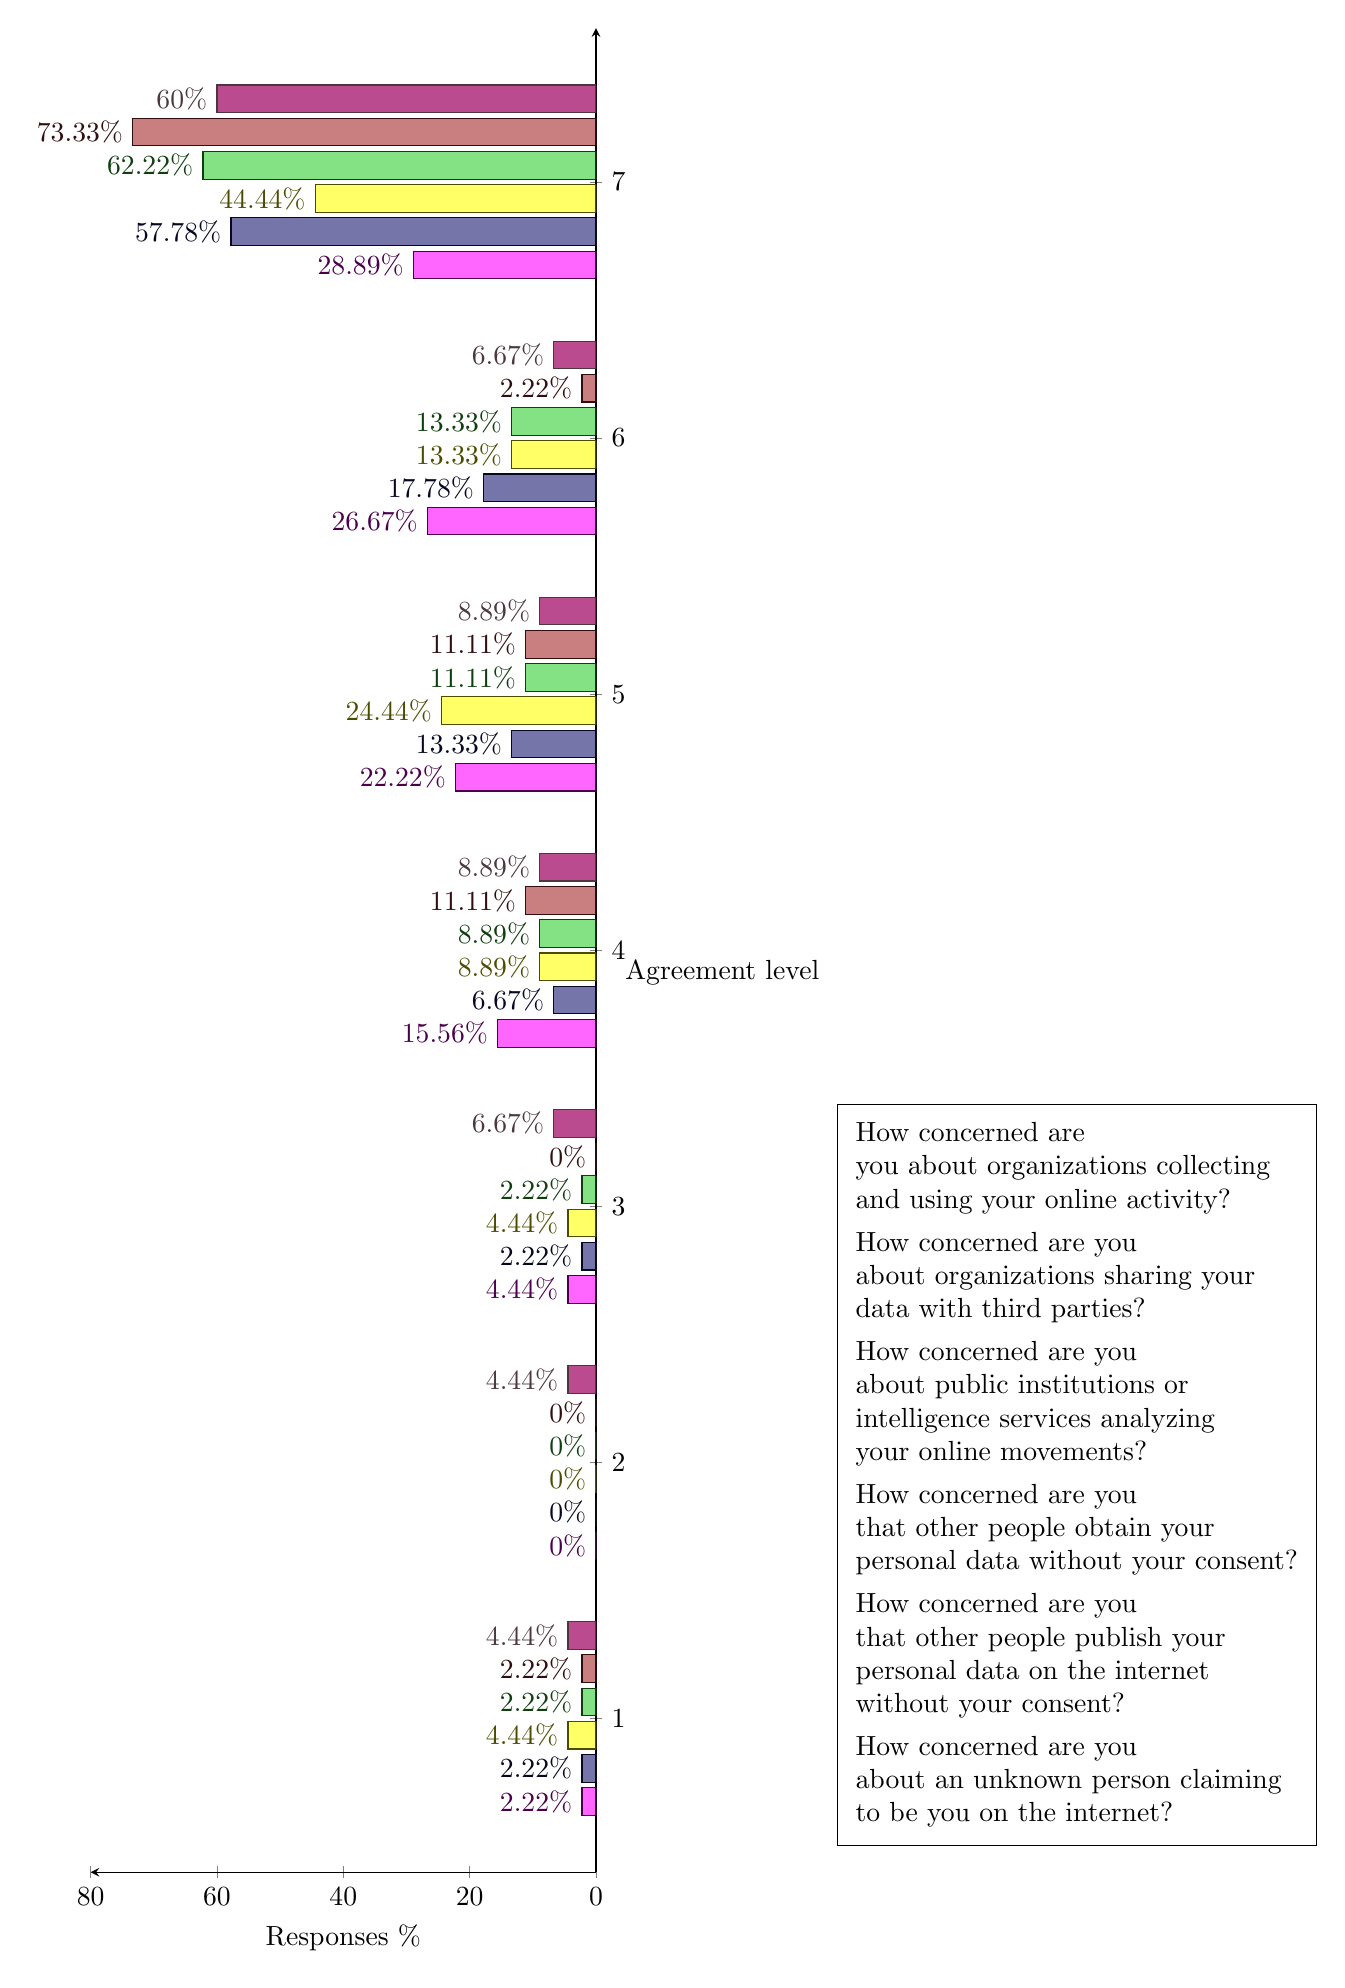
\begin{tikzpicture}[rotate=90]
            \tikzset{
                legendmatrix/.style={% style for legends
                    draw,% draw a border for the legend
                    outer sep=.3333em,% additional space to the axis label
                    nodes={rotate=0,anchor=base west,outer sep=0pt},% rotate the nodes inside the matrix
                    /pgfplots/every crossref picture/.append style={rotate=0,yshift=.75ex}% rotate the legend images
                }
            }
            \begin{axis}[
                height=8cm,
                width=25cm,
                ybar,
                bar width=10pt,
                ymin=0,
                ymax=80,
                xtick=data,
                axis x line=bottom,
                axis y line=left,
                enlarge x limits=0.1,
                xticklabel style={rotate=270},
                yticklabel style={rotate=270},
                ylabel style = {rotate=180,name=ylabel2},
                xlabel style = {rotate=270,at={(0.5,-0.25)},anchor=north},
                ylabel={Responses \%},
                xlabel={Agreement level},
                nodes near coords={\pgfmathprintnumber\pgfplotspointmeta\%},
                every node near coord/.append style={rotate=270, anchor=east},
                % legend style={at={(0.5,0.8)},anchor=south}
            ]
                \addplot[Magenta!30!black,fill=Magenta!60!white] coordinates {(1,2.22) (2,0) (3,4.44) (4,15.56) (5,22.22) (6,26.67) (7,28.89)};\label{plot:organizations_collecting_using_online_activity}
                % \addlegendentry{How concerned are you about organizations collecting and using your online activity?}
                \addplot[MidnightBlue!30!black,fill=MidnightBlue!60!white] coordinates {(1,2.22) (2,0) (3,2.22) (4,6.67) (5,13.33) (6,17.78) (7,57.78)};\label{plot:organizations_sharing_third_parties}
                % \addlegendentry{How concerned are you about organizations sharing your data with third parties?}
                \addplot[Yellow!30!black,fill=Yellow!60!white] coordinates {(1,4.44) (2,0) (3,4.44) (4,8.89) (5,24.44) (6,13.33) (7,44.44)};\label{plot:public_institutions_analyzing_online_movements}
                % \addlegendentry{How concerned are you about public institutions or intelligence services analyzing your online movements?}
                \addplot[LimeGreen!30!black,fill=LimeGreen!60!white] coordinates {(1,2.22) (2,0) (3,2.22) (4,8.89) (5,11.11) (6,13.33) (7,62.22)};\label{plot:other_people_your_data_without_consent}
                % \addlegendentry{How concerned are you that other people obtain your personal data without your consent?}
                \addplot[Brown!30!black,fill=Brown!60!white] coordinates {(1,2.22) (2,0) (3,0) (4,11.11) (5,11.11) (6,2.22) (7,73.33)};\label{plot:other_people_publish_your_data_without_consent}
                % \addlegendentry{How concerned are you that other people publish your personal data on the internet without your consent?}
                \addplot[RedViolet!30!black,fill=RedViolet!70!white] coordinates {(1,4.44) (2,4.44) (3,6.67) (4,8.89) (5,8.89) (6,6.67) (7,60)};\label{plot:unknown_claiming_to_be_you_internet}
                % \addlegendentry{How concerned are you about an unknown person claiming to be you on the internet?}
            \end{axis}
            \matrix[legendmatrix,at={(ylabel2.south)},anchor=west]{% legend for Plot 2
                \ref{plot:organizations_collecting_using_online_activity} & \node[align=left]{How concerned are\\you about organizations collecting\\and using your online activity?}; \\
                \ref{plot:organizations_sharing_third_parties} & \node[align=left]{How concerned are you\\about organizations sharing your\\data with third parties?}; \\
                \ref{plot:public_institutions_analyzing_online_movements} & \node[align=left]{How concerned are you\\about public institutions or\\intelligence services analyzing\\your online movements?}; \\
                \ref{plot:other_people_your_data_without_consent} & \node[align=left]{How concerned are you\\that other people obtain your\\personal data without your consent?}; \\
                \ref{plot:other_people_publish_your_data_without_consent} & \node[align=left]{How concerned are you\\that other people publish your\\personal data on the internet\\without your consent?}; \\
                \ref{plot:unknown_claiming_to_be_you_internet} & \node[align=left]{How concerned are you\\about an unknown person claiming\\to be you on the internet?}; \\
            };
        \end{tikzpicture}
        \caption{Responses related to concerns of organizations and individuals handling of private data.}
        \label{fig:concerns}
    \end{center}
    \vspace{-30pt}% Removes ``Float too large for the page'' warning
\end{figure}

% \begin{figure}
%     \begin{center}
%         \begin{tikzpicture}
%             \begin{axis}[
%                 ybar,
%                 xlabel={Agreement level},
%                 ylabel={Responses},
%                 ytick=\empty,
%                 xtick=data,
%                 axis x line=bottom,
%                 axis y line=left,
%                 enlarge x limits=0.2,
%                 bar width=20pt,
%                 nodes near coords={\pgfmathprintnumber\pgfplotspointmeta\%}
%             ]
%                 \addplot coordinates {(1,2.22) (2,0) (3,4.44) (4,15.56) (5,22.22) (6,26.67) (7,28.89)};
%             \end{axis}
%         \end{tikzpicture}
%         \caption{Responses to the question: How concerned are you about organizations collecting and using your online activity?}
%         \label{fig:concerned_organizations_collecting_activity}
%     \end{center}
% \end{figure}

% \begin{figure}
%     \begin{center}
%         \begin{tikzpicture}
%             \begin{axis}[
%                 ybar,
%                 xlabel={Agreement level},
%                 ylabel={Responses},
%                 ytick=\empty,
%                 xtick=data,
%                 axis x line=bottom,
%                 axis y line=left,
%                 enlarge x limits=0.2,
%                 bar width=20pt,
%                 nodes near coords={\pgfmathprintnumber\pgfplotspointmeta\%}
%             ]
%                 \addplot coordinates {(1,2.22) (2,0) (3,2.22) (4,6.67) (5,13.33) (6,17.78) (7,57.78)};
%             \end{axis}
%         \end{tikzpicture}
%         \caption{Responses to the question: How concerned are you about organizations sharing your data with third parties?}
%         \label{fig:concerned_organizations_sharing_data_third_parties}
%     \end{center}
% \end{figure}

% \begin{figure}
%     \begin{center}
%         \begin{tikzpicture}
%             \begin{axis}[
%                 ybar,
%                 xlabel={Agreement level},
%                 ylabel={Responses},
%                 ytick=\empty,
%                 xtick=data,
%                 axis x line=bottom,
%                 axis y line=left,
%                 enlarge x limits=0.2,
%                 bar width=20pt,
%                 nodes near coords={\pgfmathprintnumber\pgfplotspointmeta\%}
%             ]
%                 \addplot coordinates {(1,2.22) (2,0) (3,4.44) (4,6.67) (5,15.56) (6,17.78) (7,53.33)};
%             \end{axis}
%         \end{tikzpicture}
%         \caption{Responses to the question: How concerned are you about organizations tracking your online behavior and thus obtaining your personal data?}
%         \label{fig:concerned_organizations_tracking_behavior}
%     \end{center}
% \end{figure}

% \begin{figure}
%     \begin{center}
%         \begin{tikzpicture}
%             \begin{axis}[
%                 ybar,
%                 xlabel={Agreement level},
%                 ylabel={Responses},
%                 ytick=\empty,
%                 xtick=data,
%                 axis x line=bottom,
%                 axis y line=left,
%                 enlarge x limits=0.2,
%                 bar width=20pt,
%                 nodes near coords={\pgfmathprintnumber\pgfplotspointmeta\%}
%             ]
%                 \addplot coordinates {(1,4.44) (2,0) (3,4.44) (4,8.89) (5,24.44) (6,13.33) (7,44.44)};
%             \end{axis}
%         \end{tikzpicture}
%         \caption{Responses to the question: How concerned are you about public institutions or intelligence services analyzing your online movements?}
%         \label{fig:concerned_public_institutions_analyzing_online_movements}
%     \end{center}
% \end{figure}

% \begin{figure}
%     \begin{center}
%         \begin{tikzpicture}
%             \begin{axis}[
%                 ybar,
%                 xlabel={Agreement level},
%                 ylabel={Responses},
%                 ytick=\empty,
%                 xtick=data,
%                 axis x line=bottom,
%                 axis y line=left,
%                 enlarge x limits=0.2,
%                 bar width=20pt,
%                 nodes near coords={\pgfmathprintnumber\pgfplotspointmeta\%}
%             ]
%                 \addplot coordinates {(1,2.22) (2,0) (3,2.22) (4,8.89) (5,11.11) (6,13.33) (7,62.22)};
%             \end{axis}
%         \end{tikzpicture}
%         \caption{Responses to the question: How concerned are you that other people obtain your personal data without your consent?}
%         \label{fig:concerned_other_people_obtain_data_without_consent}
%     \end{center}
% \end{figure}

% \begin{figure}
%     \begin{center}
%         \begin{tikzpicture}
%             \begin{axis}[
%                 ybar,
%                 xlabel={Agreement level},
%                 ylabel={Responses},
%                 ytick=\empty,
%                 xtick=data,
%                 axis x line=bottom,
%                 axis y line=left,
%                 enlarge x limits=0.2,
%                 bar width=20pt,
%                 nodes near coords={\pgfmathprintnumber\pgfplotspointmeta\%}
%             ]
%                 \addplot coordinates {(1,4.44) (2,2.22) (3,2.22) (4,13.33) (5,22.22) (6,13.33) (7,42.22)};
%             \end{axis}
%         \end{tikzpicture}
%         \caption{Responses to the question: How concerned are you that other people find information about you online?}
%         \label{fig:concerned_other_people_find_information_you_online}
%     \end{center}
% \end{figure}

% \begin{figure}
%     \begin{center}
%         \begin{tikzpicture}
%             \begin{axis}[
%                 ybar,
%                 xlabel={Agreement level},
%                 ylabel={Responses},
%                 ytick=\empty,
%                 xtick=data,
%                 axis x line=bottom,
%                 axis y line=left,
%                 enlarge x limits=0.2,
%                 bar width=20pt,
%                 nodes near coords={\pgfmathprintnumber\pgfplotspointmeta\%}
%             ]
%                 \addplot coordinates {(1,2.22) (2,0) (3,0) (4,8.89) (5,13.33) (6,15.56) (7,60)};
%             \end{axis}
%         \end{tikzpicture}
%         \caption{Responses to the question: How concerned are you that other people are disclosing information about you without your knowledge?}
%         \label{fig:concerned_other_people_disclose_information_you_without_knowledge}
%     \end{center}
% \end{figure}

% \begin{figure}
%     \begin{center}
%         \begin{tikzpicture}
%             \begin{axis}[
%                 ybar,
%                 xlabel={Agreement level},
%                 ylabel={Responses},
%                 ytick=\empty,
%                 xtick=data,
%                 axis x line=bottom,
%                 axis y line=left,
%                 enlarge x limits=0.2,
%                 bar width=20pt,
%                 nodes near coords={\pgfmathprintnumber\pgfplotspointmeta\%}
%             ]
%                 \addplot coordinates {(1,2.22) (2,0) (3,0) (4,8.89) (5,13.33) (6,15.56) (7,60)};
%             \end{axis}
%         \end{tikzpicture}
%         \caption{Responses to the question: How concerned are you about other people sharing your personal data (photos, address, mobile phone number, etc.) with others without your consent?}
%         \label{fig:concerned_other_people_sharing_data_others_without_consent}
%     \end{center}
% \end{figure}

% \begin{figure}
%     \begin{center}
%         \begin{tikzpicture}
%             \begin{axis}[
%                 ybar,
%                 xlabel={Agreement level},
%                 ylabel={Responses},
%                 ytick=\empty,
%                 xtick=data,
%                 axis x line=bottom,
%                 axis y line=left,
%                 enlarge x limits=0.2,
%                 bar width=20pt,
%                 nodes near coords={\pgfmathprintnumber\pgfplotspointmeta\%}
%             ]
%                 \addplot coordinates {(1,2.22) (2,0) (3,4.44) (4,8.89) (5,15.56) (6,13.33) (7,55.56)};
%             \end{axis}
%         \end{tikzpicture}
%         \caption{Responses to the question: How concerned are you about other people sharing your personal data (photos, address, mobile phone number, etc.) with others without your consent?}
%         \label{fig:concerned_other_people_sharing_data_others_without_consent}
%     \end{center}
% \end{figure}

% \begin{figure}
%     \begin{center}
%         \begin{tikzpicture}
%             \begin{axis}[
%                 ybar,
%                 xlabel={Agreement level},
%                 ylabel={Responses},
%                 ytick=\empty,
%                 xtick=data,
%                 axis x line=bottom,
%                 axis y line=left,
%                 enlarge x limits=0.2,
%                 bar width=20pt,
%                 nodes near coords={\pgfmathprintnumber\pgfplotspointmeta\%}
%             ]
%                 \addplot coordinates {(1,2.22) (2,0) (3,0) (4,11.11) (5,11.11) (6,2.22) (7,73.33)};
%             \end{axis}
%         \end{tikzpicture}
%         \caption{Responses to the question: How concerned are you that other people publish your personal data (photos, address, mobile phone number, etc.) on the internet without your consent?}
%         \label{fig:concerned_other_people_publish_internet_without_consent}
%     \end{center}
% \end{figure}

% \begin{figure}
%     \begin{center}
%         \begin{tikzpicture}
%             \begin{axis}[
%                 ybar,
%                 xlabel={Agreement level},
%                 ylabel={Responses},
%                 ytick=\empty,
%                 xtick=data,
%                 axis x line=bottom,
%                 axis y line=left,
%                 enlarge x limits=0.2,
%                 bar width=20pt,
%                 nodes near coords={\pgfmathprintnumber\pgfplotspointmeta\%}
%             ]
%                 \addplot coordinates {(1,4.44) (2,4.44) (3,6.67) (4,8.89) (5,8.89) (6,6.67) (7,60)};
%             \end{axis}
%         \end{tikzpicture}
%         \caption{Responses to the question: How concerned are you about an unknown person claiming to be you on the internet?}
%         \label{fig:concerned_unknown_person_claiming_to_be_you}
%     \end{center}
% \end{figure}

% \begin{figure}
%     \begin{center}
%         \begin{tikzpicture}
%             \begin{axis}[
%                 ybar,
%                 xlabel={Agreement level},
%                 ylabel={Responses},
%                 ytick=\empty,
%                 xtick=data,
%                 axis x line=bottom,
%                 axis y line=left,
%                 enlarge x limits=0.2,
%                 bar width=20pt,
%                 nodes near coords={\pgfmathprintnumber\pgfplotspointmeta\%}
%             ]
%                 \addplot coordinates {(1,2.22) (2,4.44) (3,2.22) (4,8.89) (5,6.67) (6,11.11) (7,64.44)};
%             \end{axis}
%         \end{tikzpicture}
%         \caption{Responses to the question: How concerned are you about the possibility that someone may misuse your identity on the internet?}
%         \label{fig:concerned_someone_misuse_your_identity_internet}
%     \end{center}
% \end{figure}

% \begin{figure}
%     \centering
%     \begin{tikzpicture}
%         \pie[explode = 0.1]{35.56/I do not know,
%             11.11/No,
%             53.33/Yes}
%     \end{tikzpicture}
%     \caption{Responses to the question: If a law enforcement officer asks for your personal data, are you willing to share it?}
%     \label{fig:law_officer_share}
% \end{figure}

% \begin{figure}
%     \begin{center}
%         \begin{tikzpicture}
%             \begin{axis}[
%                 ybar,
%                 xlabel={Agreement level},
%                 ylabel={Responses},
%                 ytick=\empty,
%                 xtick=data,
%                 axis x line=bottom,
%                 axis y line=left,
%                 enlarge x limits=0.2,
%                 bar width=20pt,
%                 nodes near coords={\pgfmathprintnumber\pgfplotspointmeta\%}
%             ]
%                 \addplot coordinates {(1,4.44) (2,17.78) (3,13.33) (4,26.67) (5,8.89) (6,11.11) (7,17.78)};
%             \end{axis}
%         \end{tikzpicture}
%         \caption{Responses to the question: Do you usually answer online questionnaires when they are requested?}
%         \label{fig:answer_online_questionnaires}
%     \end{center}
% \end{figure}

% \begin{figure}
%     \begin{center}
%         \begin{tikzpicture}
%             \begin{axis}[
%                 ybar,
%                 xlabel={Agreement level},
%                 ylabel={Responses},
%                 ytick=\empty,
%                 xtick=data,
%                 axis x line=bottom,
%                 axis y line=left,
%                 enlarge x limits=0.2,
%                 bar width=20pt,
%                 nodes near coords={\pgfmathprintnumber\pgfplotspointmeta\%}
%             ]
%                 \addplot coordinates {(1,35.56) (2,26.67) (3,8.89) (4,13.33) (5,8.89) (6,4.44) (7,2.22)};
%             \end{axis}
%         \end{tikzpicture}
%         \caption{Responses to the question: When answering questionnaires, do you enter any false/incorrect information?}
%         \label{fig:questionnaires_incorrect_information}
%     \end{center}
% \end{figure}

The majority of participants admitted to inputting varying amounts of
incorrect information, with only 15.56\% of participants claiming to never
have entered fake information when setting up an account on a platform,
and 6.67\% said they always do, as demonstrated in Figure \ref{fig:creating_account_false_data}.
The most typical inaccurate information
entered by participants concerns their age, phone number, complete name,
birthday, electronic mail, username, home address and country of citizenship.
The most common reasons participants give for entering this false
information are when creating a temporary account or they
find that the information is not relevant, some stated that they do
not want to provide any information that may be used to identify them.

\begin{figure}[H]
    \begin{center}
        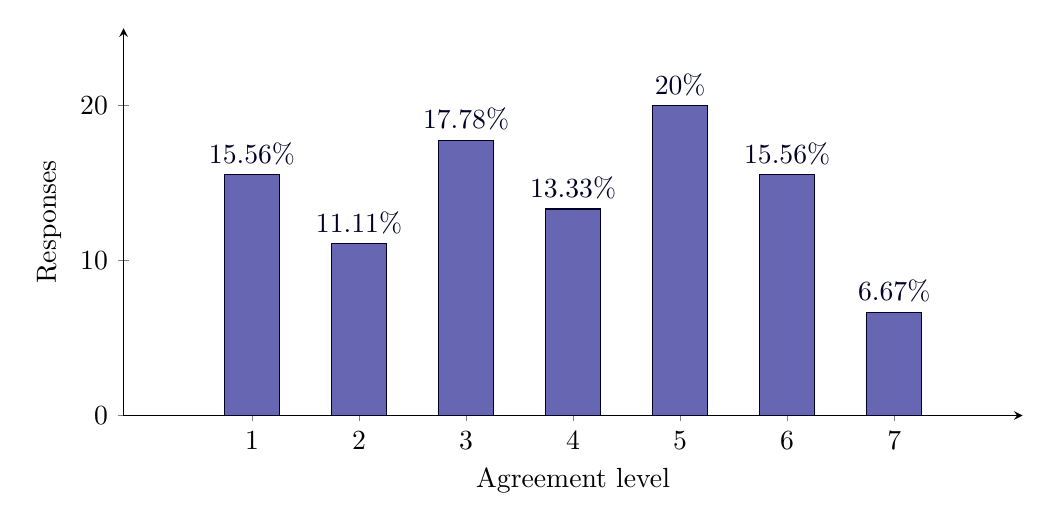
\begin{tikzpicture}
            \begin{axis}[
                height=6.5cm,
                width=13cm,
                ybar,
                xlabel={Agreement level},
                ylabel={Responses},
                ymin=0,
                ymax=25,
                % ytick=\empty,
                xtick=data,
                axis x line=bottom,
                axis y line=left,
                enlarge x limits=0.2,
                bar width=20pt,
                nodes near coords={\pgfmathprintnumber\pgfplotspointmeta\%}
            ]
                \addplot[NavyBlue!30!black,fill=NavyBlue!60!white] coordinates {(1,15.56) (2,11.11) (3,17.78) (4,13.33) (5,20) (6,15.56) (7,6.67)};
            \end{axis}
        \end{tikzpicture}
        \caption{Responses regarding the input of false personal data when creating an account on an online platform.}
        \label{fig:creating_account_false_data}
    \end{center}
\end{figure}

% \begin{figure}
%     \begin{center}
%         \begin{tikzpicture}
%             \begin{axis}[
%                 ybar,
%                 xlabel={Agreement level},
%                 ylabel={Responses},
%                 ytick=\empty,
%                 xtick=data,
%                 axis x line=bottom,
%                 axis y line=left,
%                 enlarge x limits=0.2,
%                 bar width=20pt,
%                 nodes near coords={\pgfmathprintnumber\pgfplotspointmeta\%}
%             ]
%                 \addplot coordinates {(1,0) (2,0) (3,2.22) (4,26.67) (5,17.78) (6,15.56) (7,37.78)};
%             \end{axis}
%         \end{tikzpicture}
%         \caption{Responses to the question: Can the data I disclose serve to create a profile of my online habits?}
%         \label{fig:data_disclose_create_profile}
%     \end{center}
% \end{figure}

% \begin{figure}
%     \centering
%     \begin{tikzpicture}
%         \pie[explode = 0.1]{20/I do not know,
%             4.44/No,
%             75.56/Yes}
%     \end{tikzpicture}
%     \caption{Responses to the question: ``The information I disclose on the internet can serve to identify me''. Do you agree with this statement?}
%     \label{fig:information_disclose_internet_identify_me}
% \end{figure}

Most participants are unaware of how digital data flows, as 82.22\% state
being unfamiliar with data brokers, according to Figure \ref{fig:aware_data_brokers}.
But they are aware that organisations collect their private data and use it
in various ways, even without knowing exactly what they do with the data
according to previous responses. If more individuals were aware of the function
of a data broker, which plays an important role on data flow and can be an individual
or a company which specializes in collecting and selling private data, their decisions
undoubtedly be affected by this knowledge.

\begin{figure}[H]
    \centering
    \begin{tikzpicture}
        \pie[explode = 0.1,
            color={RedOrange!70,JungleGreen!70}
            ]{82.22/No,
            17.78/Yes}
    \end{tikzpicture}
    \caption{Awareness of data brokers.}
    \label{fig:aware_data_brokers}
\end{figure}

In terms of \DTLassign{acronyms}{14}{\acronym=Acronym}\hyperlink{\acronym}{\acronym} usage and literacy, about 2/3 of the participants have interacted in
some way with a device, and from those who have used an \DTLassign{acronyms}{14}{\acronym=Acronym}\hyperlink{\acronym}{\acronym} device, only close
to a third (35.56\%) actually have a device in their homes, as depicted on
Figure \ref{fig:internet_of_things_device_usage}. Even though most participants
have interacted with an \DTLassign{acronyms}{14}{\acronym=Acronym}\hyperlink{\acronym}{\acronym} device they had trouble actually explaining what Internet
of Things actually is. When asked to describe it, 48\% of the participants
wrote some kind of ``do not know'' variation, from the other 52\% that gave
a more elaborate answer 70\% gave a generic answer that could be applied to
a number of things, some described it like objects that are connected
to the internet. Only two participants managed to describe \DTLassign{acronyms}{14}{\acronym=Acronym}\hyperlink{\acronym}{\acronym} accurately.
Most participants know devices that can be characterized as belonging to
the Internet of Things like smart homes devices, including smart
appliances like fridges, smart locks or virtual assistants that
function with natural language commands, so even though the majority
of respondents do not know how to define they can recognize \DTLassign{acronyms}{14}{\acronym=Acronym}\hyperlink{\acronym}{\acronym} devices.

\begin{figure}[H]
    \begin{center}
        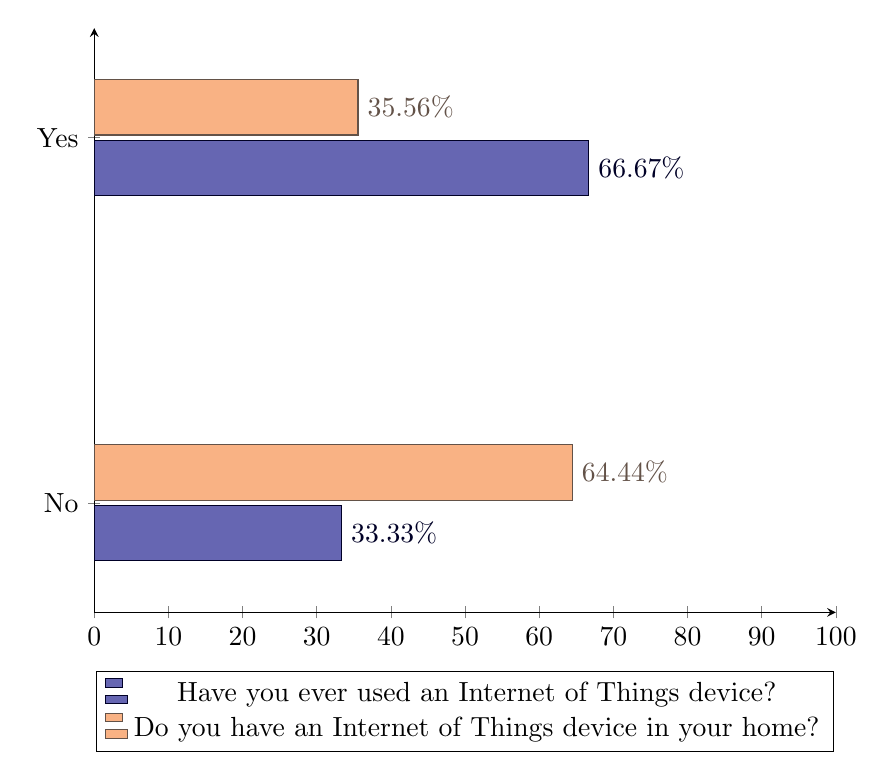
\begin{tikzpicture}
            \begin{axis}[
                height=9cm,
                width=11cm,
                xbar,
                symbolic y coords={No,Yes},
                bar width=20pt,
                ytick=data,
                axis x line=bottom,
                axis y line=left,
                xmin=0,
                xmax=100,
                enlarge y limits=0.3,
                nodes near coords={\pgfmathprintnumber\pgfplotspointmeta\%},
                legend style={at={(0.5,-0.1)},anchor=north}
            ]
                \addplot[NavyBlue!30!black,fill=NavyBlue!60!white] coordinates {(33.33,No) (66.67,Yes)};
                \addlegendentry{Have you ever used an Internet of Things device?}
                \addplot[Peach!30!black,fill=Peach!60!white] coordinates {(64.44,No) (35.56,Yes)};
                \addlegendentry{Do you have an Internet of Things device in your home?}
            \end{axis}
        \end{tikzpicture}
        \caption{Participant responses related to IoT usage.}
        \label{fig:internet_of_things_device_usage}
    \end{center}
\end{figure}

% \begin{figure}
%     \centering
%     \begin{tikzpicture}
%         \pie[explode = 0.1]{33.33/No,
%             66.67/Yes}
%     \end{tikzpicture}
%     \caption{Responses to the question: Have you ever used an Internet of Things device (smartwatch, contactless cards, air or sea traffic applications)?}
%     \label{fig:ever_used_internet_of_things_device}
% \end{figure}

% \begin{figure}
%     \centering
%     \begin{tikzpicture}
%         \pie[explode = 0.1]{64.44/No,
%             35.56/Yes}
%     \end{tikzpicture}
%     \caption{Responses to the question: Do you have an Internet of Things device in your home (assistants like Alexa, smart lock, video surveillance, etc.)?}
%     \label{fig:have_internet_of_things_device}
% \end{figure}

Familiarity with \DTLassign{acronyms}{14}{\acronym=Acronym}\hyperlink{\acronym}{\acronym} devices does not imply understanding of \DTLassign{acronyms}{14}{\acronym=Acronym}\hyperlink{\acronym}{\acronym} systems
or the majority of \DTLassign{acronyms}{14}{\acronym=Acronym}\hyperlink{\acronym}{\acronym} related concepts or terms,
as illustrated in Figure \ref{fig:familiar_terms_iot},
the most recognized terms are the ones who have more visibility
in everyday life like smart home, smart vehicle or fully autonomous car.
Esoteric terms like the ones describing networks or protocols are mostly
unknown to most respondents, only to those that have certain
qualifications or who work in \DTLassign{acronyms}{13}{\acronym=Acronym}\hyperlink{\acronym}{\acronym} or similar areas have knowledge of these concepts.

\begin{figure}[H]
    \begin{center}
        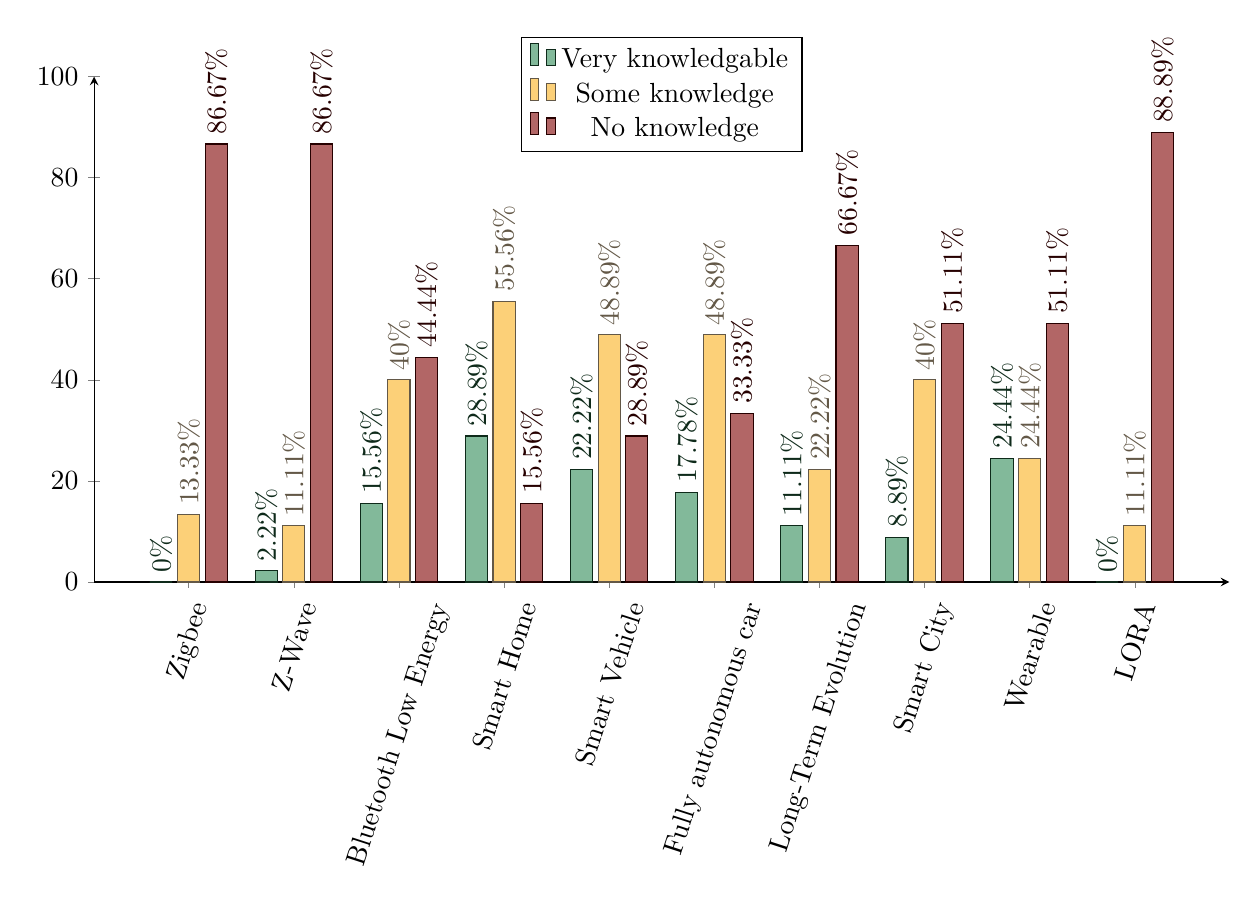
\begin{tikzpicture}
            \begin{axis}[
                height=8cm,
                width=16cm,
                symbolic x coords={Zigbee, Z-Wave,Bluetooth Low Energy,Smart Home,Smart Vehicle,Fully autonomous car,Long-Term Evolution,Smart City,Wearable,LORA},
                ybar,
                bar width=8pt,
                ymin=0,
                ymax=100,
                xticklabel style={rotate=72},
                axis x line=bottom,
                axis y line=left,
                enlarge x limits=0.1,
                nodes near coords={\pgfmathprintnumber\pgfplotspointmeta\%},
                every node near coord/.append style={rotate=90, anchor=west},
                legend style={at={(0.5,0.85)},anchor=south}
            ]
                \addplot[SeaGreen!30!black,fill=SeaGreen!60!white] coordinates {(Zigbee,0) (Z-Wave,2.22) (Bluetooth Low Energy,15.56) (Smart Home,28.89) (Smart Vehicle,22.22) (Fully autonomous car,17.78) (Long-Term Evolution,11.11) (Smart City,8.89) (Wearable,24.44) (LORA,0)};
                \addlegendentry{Very knowledgable}
                \addplot[Dandelion!30!black,fill=Dandelion!60!white] coordinates {(Zigbee,13.33) (Z-Wave,11.11) (Bluetooth Low Energy,40) (Smart Home,55.56) (Smart Vehicle,48.89) (Fully autonomous car,48.89) (Long-Term Evolution,22.22) (Smart City,40) (Wearable,24.44) (LORA,11.11)};
                \addlegendentry{Some knowledge}
                \addplot[Maroon!30!black,fill=Maroon!60!white] coordinates {(Zigbee,86.67) (Z-Wave,86.67) (Bluetooth Low Energy,44.44) (Smart Home,15.56) (Smart Vehicle,28.89) (Fully autonomous car,33.33) (Long-Term Evolution,66.67) (Smart City,51.11) (Wearable,51.11) (LORA,88.89)};
                \addlegendentry{No knowledge}
            \end{axis}
        \end{tikzpicture}
        \caption{Familiarity with IoT terms.}
        \label{fig:familiar_terms_iot}
    \end{center}
\end{figure}

\subsection{Stage 2: Application}

The usability test was given to each participant before giving a basic debrief
of what the application is about. Participants would score the overall difficulty
after performing each task. When participants first used the application, they
found it to be similar to other mapping applications, they had some difficulty
adjusting to the application's function but were quick to adapt. The tasks consisted
of navigating the application and performing certain actions such as creating
a user account or adding an \DTLassign{acronyms}{14}{\acronym=Acronym}\hyperlink{\acronym}{\acronym} device, these tasks include navigating to the \DTLassign{acronyms}{14}{\acronym=Acronym}\hyperlink{\acronym}{\acronym} devices
page; looking up information about any one particular device; navigating to the
homepage and performing the same action as the previous step; looking up
general information about the application itself; creating an account;
looking up information about privacy, the Internet of Things, and how
to add a device to the application; adding an \DTLassign{acronyms}{14}{\acronym=Acronym}\hyperlink{\acronym}{\acronym} device; and finally,
updating an \DTLassign{acronyms}{14}{\acronym=Acronym}\hyperlink{\acronym}{\acronym} device. The first tests revealed to be
somewhat difficult because of a language barrier, the application, at the
time, was only available in english and the participants had a rough grasp of it.
It was still possible to conduct the tests after translating everything the application
did.
Some participants struggled to
find the \DTLassign{acronyms}{14}{\acronym=Acronym}\hyperlink{\acronym}{\acronym} devices on the application at the start, but eventually it
became second nature. There was also some difficulty in adding an \DTLassign{acronyms}{14}{\acronym=Acronym}\hyperlink{\acronym}{\acronym} device,
mostly from older participants. Participants who were already comfortable with
technology or who had worked in fields connected to \DTLassign{acronyms}{13}{\acronym=Acronym}\hyperlink{\acronym}{\acronym} did not have any trouble
completing each task, although only one of these participants had some knowledge
of \DTLassign{acronyms}{14}{\acronym=Acronym}\hyperlink{\acronym}{\acronym}.

Figure \ref{fig:single_ease_questions} shows the average responses of the
single ease questions. Participants found task 8, on average, to be the most difficult,
in which they were asked to add an \DTLassign{acronyms}{14}{\acronym=Acronym}\hyperlink{\acronym}{\acronym} device to the application. The
participants that had the most difficulty also had very little knowledge
about \DTLassign{acronyms}{14}{\acronym=Acronym}\hyperlink{\acronym}{\acronym}, which made the task more difficult; they were unsure what type
of information to insert, despite the fact that hints are provided in the
form and the user is warned if any information entered is erroneous. In
general, the lack awareness about \DTLassign{acronyms}{14}{\acronym=Acronym}\hyperlink{\acronym}{\acronym} correlates with the challenge faced when
performing some tasks. The older age group of participants struggled more on the
tests while the younger participants demonstrated no noticeable difficulties.
All usability tests were conducted in the same manner, as in, on each session
a debrief was given about the purpose of the work and the application, next
the participant completed the survey, if it was not previously filled, then there
was some discussion about the survey and the application and the usability
test would start proper. On this phase every participant did the exact same
usability test, meaning the tasks were not randomized on each session, this
fact might have created some bias on the analysis of the tests.

\begin{figure}[H]
    \begin{center}
        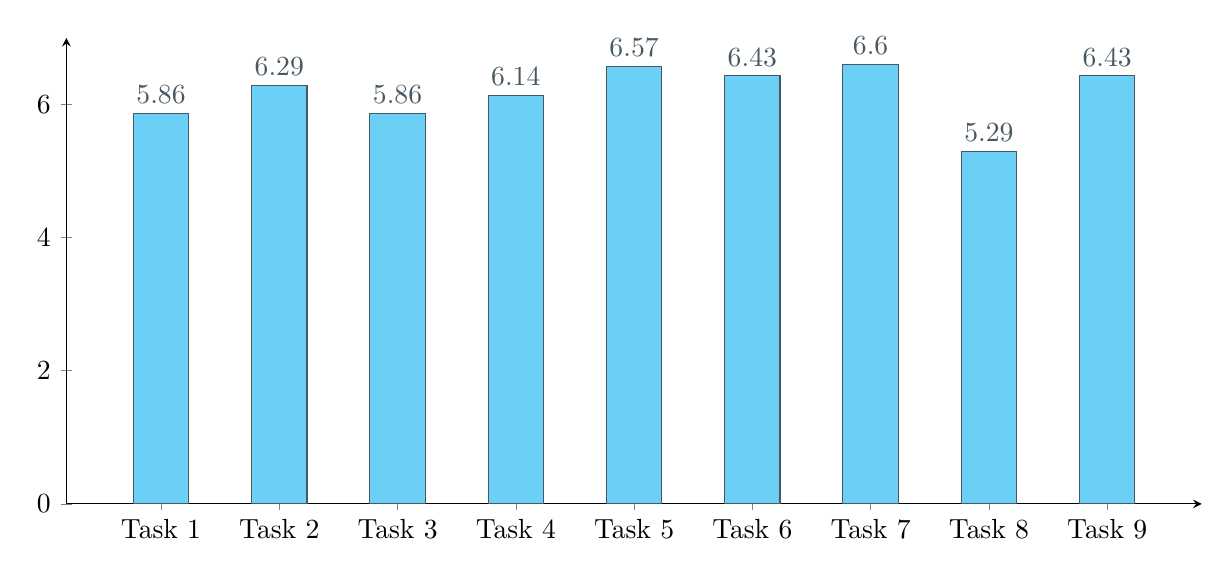
\begin{tikzpicture}
            \begin{axis}[
                height=7.5cm,
                width=16cm,
                ybar,
                ymin=0,
                ymax=7,
                symbolic x coords={Task 1,Task 2,Task 3,Task 4,Task 5,Task 6,Task 7,Task 8,Task 9},
                % ytick=\empty,
                xtick=data,
                axis x line=bottom,
                axis y line=left,
                enlarge x limits=0.1,
                bar width=20pt,
                nodes near coords={\pgfmathprintnumber\pgfplotspointmeta}
            ]
                \addplot[ProcessBlue!30!black,fill=ProcessBlue!60!white] coordinates {(Task 1,5.86) (Task 2,6.29) (Task 3,5.86) (Task 4,6.14) (Task 5,6.57) (Task 6,6.43) (Task 7,6.6) (Task 8,5.29) (Task 9,6.43)};
            \end{axis}
        \end{tikzpicture}
        \caption{Average participant responses of the single ease questions.}
        \label{fig:single_ease_questions}
    \end{center}
\end{figure}

The \DTLassign{acronyms}{27}{\acronym=Acronym}\hyperlink{\acronym}{\acronym} was used after the participants
performed all tasks, using this system an average score of 90,95 was achieved.
In Figure \ref{fig:system_usability_scale_scores} the scores of
each participant can be seen.
The score was calculated by using the following formula:
\begin{equation}\label{sus}
    Score = \frac{\sum_{i=1}^{n}f(P_i)}{n}
\end{equation}
where $n$ is the number of participants, which in this case is equal to 7,
and $f(P)$, representing each participants' response ($P$), is noted as:
\begin{equation}\label{individual_sus}
    ((Q1-1)+(7-Q2)+(Q3-1)+(7-Q4)+(Q5-1)+(7-Q6)+(Q7-1)+(7-Q8)+(Q9-1)+(7-Q10))*\frac{5}{3}
\end{equation}
where $Q1$, $Q2$, $Q3$, $Q4$, $Q5$, $Q6$, $Q7$, $Q8$, $Q9$ and $Q10$ refers to
the score of a participant for each question.

\nameref{appendix:sus} shows the scoring in more detail.
The obtained value of 90,95 is a high score which would mean that the application provides
a good user experience, even though some users experienced some
hardships when using it when the first tests where being performed.
The feedback given by these participants helped in improving the application,
as is the example of when the application was only available in english,
now it is possible to use it in english and in portuguese, in the future
more language might be added.

\begin{figure}[H]
    \begin{center}
        \begin{tikzpicture}
            \begin{axis}[
                % width=14cm,
                % height=8cm,
                % xmin=2010,
                % xmax=2023,
                ymin=0,
                ymax=100,
                % xlabel=Year,
                % ylabel=Papers,
                axis x line=bottom,
                axis y line=left,
                enlarge x limits=0.1,
                nodes near coords={\pgfmathprintnumber\pgfplotspointmeta}
            ]
            \addplot[scatter, only marks] coordinates {(1,85) (2,90) (3,91.66666667) (4,96.66666667) (5,98.33333333) (6,96.66666667) (7,78.33333333)};
            \end{axis}
        \end{tikzpicture}
        \caption{Individual system usability scale scores.}
        \label{fig:system_usability_scale_scores}
    \end{center}
\end{figure}

An improvement to the usability tests would be to have the participation of
an expert software developer, preferably with experience in \DTLassign{acronyms}{14}{\acronym=Acronym}\hyperlink{\acronym}{\acronym} systems.
